%%
% Copyright (c) 2017 - 2019, Pascal Wagler;
% Copyright (c) 2014 - 2019, John MacFarlane
%
% All rights reserved.
%
% Redistribution and use in source and binary forms, with or without
% modification, are permitted provided that the following conditions
% are met:
%
% - Redistributions of source code must retain the above copyright
% notice, this list of conditions and the following disclaimer.
%
% - Redistributions in binary form must reproduce the above copyright
% notice, this list of conditions and the following disclaimer in the
% documentation and/or other materials provided with the distribution.
%
% - Neither the name of John MacFarlane nor the names of other
% contributors may be used to endorse or promote products derived
% from this software without specific prior written permission.
%
% THIS SOFTWARE IS PROVIDED BY THE COPYRIGHT HOLDERS AND CONTRIBUTORS
% "AS IS" AND ANY EXPRESS OR IMPLIED WARRANTIES, INCLUDING, BUT NOT
% LIMITED TO, THE IMPLIED WARRANTIES OF MERCHANTABILITY AND FITNESS
% FOR A PARTICULAR PURPOSE ARE DISCLAIMED. IN NO EVENT SHALL THE
% COPYRIGHT OWNER OR CONTRIBUTORS BE LIABLE FOR ANY DIRECT, INDIRECT,
% INCIDENTAL, SPECIAL, EXEMPLARY, OR CONSEQUENTIAL DAMAGES (INCLUDING,
% BUT NOT LIMITED TO, PROCUREMENT OF SUBSTITUTE GOODS OR SERVICES;
% LOSS OF USE, DATA, OR PROFITS; OR BUSINESS INTERRUPTION) HOWEVER
% CAUSED AND ON ANY THEORY OF LIABILITY, WHETHER IN CONTRACT, STRICT
% LIABILITY, OR TORT (INCLUDING NEGLIGENCE OR OTHERWISE) ARISING IN
% ANY WAY OUT OF THE USE OF THIS SOFTWARE, EVEN IF ADVISED OF THE
% POSSIBILITY OF SUCH DAMAGE.
%%

%%
% This is the Eisvogel pandoc LaTeX template.
%
% For usage information and examples visit the official GitHub page:
% https://github.com/Wandmalfarbe/pandoc-latex-template
%%

% Options for packages loaded elsewhere
\PassOptionsToPackage{unicode}{hyperref}
\PassOptionsToPackage{hyphens}{url}
\PassOptionsToPackage{dvipsnames,svgnames*,x11names*,table}{xcolor}
%
\documentclass[
  a4paper,
,tablecaptionabove
]{scrartcl}
\usepackage{lmodern}
\usepackage{setspace}
\setstretch{1.2}
\usepackage{amssymb,amsmath}
\usepackage{ifxetex,ifluatex}
\ifnum 0\ifxetex 1\fi\ifluatex 1\fi=0 % if pdftex
  \usepackage[T1]{fontenc}
  \usepackage[utf8]{inputenc}
  \usepackage{textcomp} % provide euro and other symbols
\else % if luatex or xetex
  \usepackage{unicode-math}
  \defaultfontfeatures{Scale=MatchLowercase}
  \defaultfontfeatures[\rmfamily]{Ligatures=TeX,Scale=1}
\fi
% Use upquote if available, for straight quotes in verbatim environments
\IfFileExists{upquote.sty}{\usepackage{upquote}}{}
\IfFileExists{microtype.sty}{% use microtype if available
  \usepackage[]{microtype}
  \UseMicrotypeSet[protrusion]{basicmath} % disable protrusion for tt fonts
}{}
\makeatletter
\renewcommand{\verbatim@font}{\ttfamily\scriptsize}
\makeatother
\makeatletter
\@ifundefined{KOMAClassName}{% if non-KOMA class
  \IfFileExists{parskip.sty}{%
    \usepackage{parskip}
  }{% else
    \setlength{\parindent}{0pt}
    \setlength{\parskip}{6pt plus 2pt minus 1pt}}
}{% if KOMA class
  \KOMAoptions{parskip=half}}
\makeatother
\usepackage{xcolor}
\definecolor{default-linkcolor}{HTML}{A50000}
\definecolor{default-filecolor}{HTML}{A50000}
\definecolor{default-citecolor}{HTML}{4077C0}
\definecolor{default-urlcolor}{HTML}{4077C0}
\IfFileExists{xurl.sty}{\usepackage{xurl}}{} % add URL line breaks if available
\IfFileExists{bookmark.sty}{\usepackage{bookmark}}{\usepackage{hyperref}}
\hypersetup{
  pdftitle={Técnicas de soft computing para Aprendizaje y Optimización},
  pdfauthor={Francisco Luque Sánchez},
  colorlinks=true,
  linkcolor=default-linkcolor,
  filecolor=default-filecolor,
  citecolor=default-citecolor,
  urlcolor=blue,
  breaklinks=true,
  pdfcreator={LaTeX via pandoc with the Eisvogel template}}
\urlstyle{same} % disable monospaced font for URLs
\usepackage[margin=2.5cm,includehead=true,includefoot=true,centering,]{geometry}
% add backlinks to footnote references, cf. https://tex.stackexchange.com/questions/302266/make-footnote-clickable-both-ways
\usepackage{footnotebackref}
\usepackage{graphicx,grffile}
\makeatletter
\def\maxwidth{\ifdim\Gin@nat@width>\linewidth\linewidth\else\Gin@nat@width\fi}
\def\maxheight{\ifdim\Gin@nat@height>\textheight\textheight\else\Gin@nat@height\fi}
\makeatother
% Scale images if necessary, so that they will not overflow the page
% margins by default, and it is still possible to overwrite the defaults
% using explicit options in \includegraphics[width, height, ...]{}
\setkeys{Gin}{width=\maxwidth,height=\maxheight,keepaspectratio}
\setlength{\emergencystretch}{3em}  % prevent overfull lines
\providecommand{\tightlist}{%
  \setlength{\itemsep}{0pt}\setlength{\parskip}{0pt}}
\setcounter{secnumdepth}{3}

% Make use of float-package and set default placement for figures to H.
% The option H means 'PUT IT HERE' (as  opposed to the standard h option which means 'You may put it here if you like').
\usepackage{float}
\floatplacement{figure}{H}

\usepackage[ruled,vlined,linesnumbered]{algorithm2e}
\usepackage{subcaption}
\usepackage{booktabs}
\usepackage{longtable}

\title{Técnicas de soft computing para Aprendizaje y Optimización}
\usepackage{etoolbox}
\makeatletter
\providecommand{\subtitle}[1]{% add subtitle to \maketitle
  \apptocmd{\@title}{\par {\large #1 \par}}{}{}
}
\makeatother
\subtitle{Trabajo Final - Optimización basada en colmenas}
\author{Francisco Luque Sánchez}
\date{21/05/2020}



%%
%% added
%%

%
% language specification
%
% If no language is specified, use English as the default main document language.
%

\ifnum 0\ifxetex 1\fi\ifluatex 1\fi=0 % if pdftex
  \usepackage[shorthands=off,main=english]{babel}
\else
    % Workaround for bug in Polyglossia that breaks `\familydefault` when `\setmainlanguage` is used.
  % See https://github.com/Wandmalfarbe/pandoc-latex-template/issues/8
  % See https://github.com/reutenauer/polyglossia/issues/186
  % See https://github.com/reutenauer/polyglossia/issues/127
  \renewcommand*\familydefault{\sfdefault}
    % load polyglossia as late as possible as it *could* call bidi if RTL lang (e.g. Hebrew or Arabic)
  \usepackage{polyglossia}
  \setmainlanguage[]{english}
\fi



%
% for the background color of the title page
%
\usepackage{pagecolor}
\usepackage{afterpage}
\usepackage{tikz}
\usepackage[margin=2.5cm,includehead=true,includefoot=true,centering]{geometry}

%
% break urls
%
\PassOptionsToPackage{hyphens}{url}

%
% When using babel or polyglossia with biblatex, loading csquotes is recommended
% to ensure that quoted texts are typeset according to the rules of your main language.
%
\usepackage{csquotes}

%
% captions
%
\definecolor{caption-color}{HTML}{777777}
\usepackage[font={stretch=1.2}, textfont={color=caption-color}, position=top, skip=4mm, labelfont=bf, singlelinecheck=false, justification=raggedright]{caption}
\setcapindent{0em}

%
% blockquote
%
\definecolor{blockquote-border}{RGB}{221,221,221}
\definecolor{blockquote-text}{RGB}{119,119,119}
\usepackage{mdframed}
\newmdenv[rightline=false,bottomline=false,topline=false,linewidth=3pt,linecolor=blockquote-border,skipabove=\parskip]{customblockquote}
\renewenvironment{quote}{\begin{customblockquote}\list{}{\rightmargin=0em\leftmargin=0em}%
\item\relax\color{blockquote-text}\ignorespaces}{\unskip\unskip\endlist\end{customblockquote}}

%
% Source Sans Pro as the de­fault font fam­ily
% Source Code Pro for monospace text
%
% 'default' option sets the default
% font family to Source Sans Pro, not \sfdefault.
%
\ifnum 0\ifxetex 1\fi\ifluatex 1\fi=0 % if pdftex
    \usepackage[default]{sourcesanspro}
  \usepackage{sourcecodepro}
  \else % if not pdftex
    \usepackage[default]{sourcesanspro}
  \usepackage{sourcecodepro}

  % XeLaTeX specific adjustments for straight quotes: https://tex.stackexchange.com/a/354887
  % This issue is already fixed (see https://github.com/silkeh/latex-sourcecodepro/pull/5) but the
  % fix is still unreleased.
  % TODO: Remove this workaround when the new version of sourcecodepro is released on CTAN.
  \ifxetex
    \makeatletter
    \defaultfontfeatures[\ttfamily]
      { Numbers   = \sourcecodepro@figurestyle,
        Scale     = \SourceCodePro@scale,
        Extension = .otf }
    \setmonofont
      [ UprightFont    = *-\sourcecodepro@regstyle,
        ItalicFont     = *-\sourcecodepro@regstyle It,
        BoldFont       = *-\sourcecodepro@boldstyle,
        BoldItalicFont = *-\sourcecodepro@boldstyle It ]
      {SourceCodePro}
    \makeatother
  \fi
  \fi

%
% heading color
%
\definecolor{heading-color}{RGB}{40,40,40}
\addtokomafont{section}{\color{heading-color}}
% When using the classes report, scrreprt, book,
% scrbook or memoir, uncomment the following line.
%\addtokomafont{chapter}{\color{heading-color}}

%
% variables for title and author
%
\usepackage{titling}
\title{Técnicas de soft computing para Aprendizaje y Optimización}
\author{Francisco Luque Sánchez}

%
% tables
%

%
% remove paragraph indention
%
\setlength{\parindent}{0pt}
\setlength{\parskip}{6pt plus 2pt minus 1pt}
\setlength{\emergencystretch}{3em}  % prevent overfull lines

%
%
% Listings
%
%


%
% header and footer
%
\usepackage{fancyhdr}

\fancypagestyle{eisvogel-header-footer}{
  \fancyhead{}
  \fancyfoot{}
  \lhead[21/05/2020]{Técnicas de soft computing para Aprendizaje y Optimización}
  \chead[]{}
  \rhead[Técnicas de soft computing para Aprendizaje y Optimización]{21/05/2020}
  \lfoot[\thepage]{Francisco Luque Sánchez}
  \cfoot[]{}
  \rfoot[Francisco Luque Sánchez]{\thepage}
  \renewcommand{\headrulewidth}{0.4pt}
  \renewcommand{\footrulewidth}{0.4pt}
}
\pagestyle{eisvogel-header-footer}

%%
%% end added
%%

\begin{document}

%%
%% begin titlepage
%%
\begin{titlepage}
\newgeometry{top=2cm, right=4cm, bottom=3cm, left=4cm}
\tikz[remember picture,overlay] \node[inner sep=0pt] at (current page.center){\includegraphics[width=\paperwidth,height=\paperheight]{background8.pdf}};
\newcommand{\colorRule}[3][black]{\textcolor[HTML]{#1}{\rule{#2}{#3}}}
\begin{flushleft}
\noindent
\\[-1em]
\color[HTML]{5F5F5F}
\makebox[0pt][l]{\colorRule[435488]{1.3\textwidth}{4pt}}
\par
\noindent

% The titlepage with a background image has other text spacing and text size
{
  \setstretch{2}
  \vfill
  \vskip -8em
  \noindent {\huge \textbf{\textsf{Técnicas de soft computing para Aprendizaje y Optimización}}}
    \vskip 1em
  {\Large \textsf{Trabajo Final - Optimización basada en colmenas}}
    \vskip 2em
  \noindent {\Large \textsf{Francisco Luque Sánchez} \vskip 0.6em \textsf{21/05/2020}}
  \vfill
}


\end{flushleft}
\end{titlepage}
\restoregeometry

%%
%% end titlepage
%%



\renewcommand*\contentsname{Índice}
{
\hypersetup{linkcolor=}
\setcounter{tocdepth}{2}
\tableofcontents
\newpage
}
\hypertarget{introducciuxf3n}{%
\section{Introducción}\label{introducciuxf3n}}

En este trabajo se va a desarrollar un estudio comparativo sobre
algoritmos basados en colmenas para optimización numérica (\emph{swarm
optimization}). Estos algoritmos utilizan un modelo de optimización
numérica basado en evaluación y búsqueda de soluciones no analítico. El
funcionamiento de estos algoritmos se basa en la exploración del espacio
de soluciones por medio de una población en la que cada individuo
representa una solución posible. Estas soluciones se van desplazando por
el espacio, utilizando la información del resto para explorar.

En particular, estaremos interesados en el empleo de estos modelos para
la minimización de funciones reales y unimodales de variable real. Esto
significa que tendremos una función \(f: \mathbb{R}^D \to \mathbb{R}\),
y estaremos interesados en encontrar \(\mathbf{x}^* \in \mathbb{R}^D\)
tal que
\(f(\mathbf{x}^*) \leq f(\mathbf{x}) \; \forall \; \mathbf{x} \in \mathbb{R}^D\).
Nuestra intención es, por tanto, encontrar el mínimo de la función \(f\)
dentro de nuestro espacio de búsqueda.

Para realizar nuestro estudio, utilizaremos un conjunto de funciones
reales de variable real, que nos permitirán estudiar la calidad de
nuestros algoritmos sobre las mismas. Concretamente, utilizaremos el
conjunto de funciones de la competición CEC 2014 en optimización de
parámetros reales de objetivo único (Por su nombre en inglés, \emph{CEC
2014 Competition on Real-Parameter Single Objective Optimization}).

Comenzamos definiendo un marco teórico genérico para el desarrollo de
algoritmos basados en enjambres.

\hypertarget{algoritmos-basados-en-enjambres}{%
\section{Algoritmos basados en
enjambres}\label{algoritmos-basados-en-enjambres}}

En esta sección, daremos un marco teórico para el desarrollo de
algoritmos basados en enjambres.

Sea \(f: \mathbb{R}^D \to \mathbb{R}\) una función de coste a minimizar
(claramente, si el problema a resolver es un problema de maximización,
es suficiente con tomar \(g(\mathbf{x}) = - f(\mathbf{x})\) y minimizar
la función \(g\)). La función \(f\) toma como argumento un vector
\(D\)-dimensional de valores reales y produce como resultado un valor
real. Supongamos que el gradiente de la función \(f\) no puede ser
calculado, y por tanto no podremos utilizar técnicas clásicas de
optimización por métodos analíticos. Nuestro objetivo es encontrar el
mínimo global de la función \(f\), esto es, encontrar
\(\mathbf{x}^* \in \mathbb{R}^D\) tal que
\(\forall \mathbf{x} \in \mathbb{R}^D\) se tiene que
\(f(\mathbf{x}^*) \leq f(\mathbf{x})\). Se dice entonces que
\(\mathbf{x}\) es un mínimo global de la función \(f\).

Sea \(S\) el enjambre de soluciones. Entonces,
\(S = \{\mathbf{x}_1, ..., \mathbf{x}_k\}\) un conjunto de \(k\)
posibles soluciones en el espacio de búsqueda, es decir,
\(\mathbf{x}_i \in \mathbb{R}^D, i=1,...,k\), las cuales se inicializan
de forma aleatoria uniforme en el espacio de búsqueda (usualmente, en
lugar de trabajar en \(\mathbb{R}^D\), trabajaremos en un subconjunto
compacto del mismo, definido como \([a, b]^D\), con
\(a, b \in \mathbb{R}, a < b\)).

\begin{algorithm}[H]
\DontPrintSemicolon
\SetAlgoLined

\BlankLine
    Inicializar aleatoriamente la población\;
    Evaluar la población con la función objetivo\;
    Obtener los mejores individuos en función de la evaluación $S_{best}$\;
    \While{No se cumpla el criterio de parada}{
        \For{Cada partícula en $S$}{
            Actualizar su posición en función de su posición actual y los individuos en $S_{best}$\;
            Evaluar la nueva solución obtenida\;
        }
        Actualizar los mejores individuos de la población en $S_{best}$\;
        Guardar el mejor individuo obtenido hasta el momento\;
    }
    Devolver el mejor individuo obtenido junto con el valor de la función de evaluación en ese punto\;
\caption{Optimización basada en enjambres}
\end{algorithm}

Por tanto, el esqueleto de un algoritmo de optimización basado en
enjambres está definido de forma genérica, y cada algoritmo particular
estará definido por una serie de parámetros que lo diferenciará del
resto. Estos parámetros son los siguientes:

\begin{itemize}
\tightlist
\item
  Condición de parada del algoritmo: Indica cuándo se considera que el
  proceso de optimización ha terminado. Usualmente se utiliza como
  condición de parada un número prefijado de evaluaciones de la función
  objetivo, y así lo tendremos definido en nuestro caso. Más adelante
  especificaremos cuál es esa condición de parada, que viene impuesta
  por el propio \emph{benchmark} de evaluación.
\item
  La forma de seleccionar los mejores individuos: En función del
  algoritmo que estemos utilizando, dicho conjunto estará formado por el
  mejor individuo de la población (aquél que consigue un menor valor de
  la función de evaluación), o un subconjunto de los mismos
\item
  Las ecuaciones de movimiento para actualizar la posición de los
  individuos: Este suele ser el principal punto de diversidad de los
  distintos algoritmos, ya que es el principal factor que define cómo se
  explora el espacio de soluciones.
\end{itemize}

Usualmente, las ecuaciones de movimiento y la forma de selección de los
mejores individuos tienen una inspiración en modelos biológicos de
comportamiento de diversas poblaciones animales, y es por esto por lo
que se le da el nombre de optimización basada en enjambres. En
particular, uno de los primeros algoritmos que se diseñaron con esta
inspiración es el que se conoce como \emph{Particle Swarm Optimization}
(PSO) (Kennedy and Eberhart 1995), los cuales tomaron como inspiración
el comportamiento social de colonias de aves y peces para su propuesta
de optimización. Desde aquel momento, se han dado nuevas propuestas
basadas en el comportamiento de otras especies, con la intención de
obtener algoritmos que obtengan mejores resultados en el proceso de
optimización, mejorando la velocidad de convergencia a buenas
soluciones, tratando de evitar que el algoritmo converja prematuramente
en mínimos locales que no son mínimos globales de la función, o buscando
robustez en el proceso de optimización (que se el resultado no sea
fuertemente dependiente de la ejecución, y se obtengan resultados
razonables en todas las ejecuciones).

En este contexto, han aparecido algoritmos con inspiraciones muy
diversas. Existen propuestas basadas en la organización de colmenas de
abejas, en las cuales las soluciones toman el rol de abejas
recolectoras, trabajadoras o reinas, propuestas basadas en colonias de
hormigas en las cuales las soluciones dejan un rastro de feromonas en
función de la calidad de las soluciones que visitan, colonias de gatos
que se distribuyen en la búsqueda de comida, etc. En particular, en este
trabajo se van a estudiar e implementar tres algoritmos, los cuales se
basan en tres poblaciones distintas; Whale Optimization Algorithm (WOA)
(Mirjalili and Lewis 2016), cuya inspiración aparece en cómo se
comunican entre sí las ballenas jorobadas en el proceso de captura de
bancos de peces, Grey Wolf Optimizer (GWO) (Mirjalili, Mirjalili, and
Lewis 2014), en el que la inspiración se toma de la caza del lobo gris,
y Moth-Flame Optimization Algorithm (MFO) (Mirjalili 2015), basado en el
movimiento de las polillas al acercarse a una fuente de luz.
Describiremos estas metaheurísticas con más detalle en secciones
posteriores.

Pasamos a continuación a describir el \emph{benchmark} sobre el que
hemos evaluado los algoritmos de optimización.

\hypertarget{cec-2014-competition-on-real-param-single-objective-optimization}{%
\section{CEC 2014 Competition on Real-Param Single Objective
Optimization}\label{cec-2014-competition-on-real-param-single-objective-optimization}}

Para comprobar la calidad de los algoritmos propuestos, se ha decidido
utilizar los mismos para resolver un problema de optimización propuesto
como competición en el congreso de computación evolutiva del IEEE del
año 2014 (CEC 2014: IEEE Congress on Evolutionary Computation) (Liang,
Qu, and Suganthan 2013). Esta competición consiste en una \emph{suite}
compuesta por 30 funciones de optimización distintas, todas ellas
definidas como una función real de variable real. La intención de este
conjunto de funciones es medir la capacidad de los algoritmos de
optimización de minimizarlas, cuando las funciones a optimizar tienen
propiedades que dificultan en gran medida la obtención del mínimo. De
esta manera, nos encontramos con funciones con múltiples mínimos
locales, grandes mesetas (zonas del espacio en el que el valor de la
función es constante o varía muy poco), funciones que toman el mínimo en
un punto rodeado por zonas en las que el valor de la función es muy
grande, funciones no derivables en todos sus puntos, etc. Además, se
definen un conjunto de funciones base, y se construyen funciones más
complejas como combinación de dichas funciones base. No entraremos en
más detalle de las 30 funciones definidas, ya que pueden consultarse las
mismas en (Liang, Qu, and Suganthan 2013), aunque a continuación
mostramos dos figuras de la representación gráfica de dos de las
funciones en dos dimensiones (la función de Ackley, función 5 a
optimizar, y la función de Rastrigin, número 8), para dar una idea del
tipo de funciones al que nos enfrentamos. Ambas imágenes han sido
extraídas de (Liang, Qu, and Suganthan 2013).

\begin{figure}[H]
\centering
\begin{subfigure}{0.5\textwidth}
 \centering
  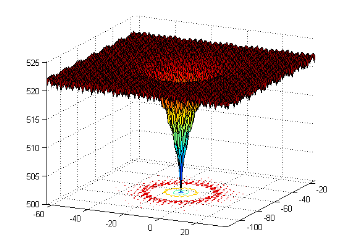
\includegraphics[width=\textwidth]{imgs/F5.png}
  \caption{Función de Ackley}
  \label{fig:sub1}
\end{subfigure}%
\begin{subfigure}{.5\textwidth}
  \centering
  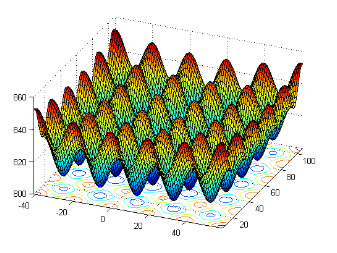
\includegraphics[width=\textwidth]{imgs/F8.png}
  \caption{Función de Rastrigin}
  \label{fig:sub2}
\end{subfigure}
\caption{Ejemplo de dos funciones extraídas del CEC2014 en dos dimensiones}
\label{fig:test}
\end{figure}

Como podemos observar en las dos imágenes anteriores, el proceso de
optimización de las mismas puede ser realmente complejo, por lo que
necesitamos algoritmos de optimización de cierta potencia para afrontar
la tarea de minimización.

Como dijimos anteriormente, el \emph{benchmark} impone ciertas
condiciones de ejecución para los problemas. Concretamente, en la
competición original se exigía resolver el problema de optimización para
las 30 funciones definidas bajo las siguientes condiciones:

\begin{itemize}
\tightlist
\item
  Dimensiones del problema: 10, 30, 50 y 100
\item
  Ejecuciones: 51 por problema
\item
  Máximo número de evaluaciones de la función objetivo: 10000
  multiplicado por el tamaño del problema (100000 para dimensión 10,
  300000 para dimensión 30, etc)
\item
  Dominio del problema: \([-100, 100]^D\), donde \(D\) es la dimensión
  del problema.
\item
  Inicialización de la población: Aleatoria uniforme en el espacio de
  búsqueda.
\end{itemize}

Como podemos observar, los requisitos de ejecución son bastante fuertes,
y nosotros relajaremos un poco las condiciones previas, debido a que no
queremos simular la competición completamente, si no hacer un estudio
comparativo entre tres algoritmos. Concretamente, sólo ejecutaremos los
problemas de tamaño 10, 30 y 50, y realizaremos 25 ejecuciones para cada
caso. De esta manera, tendremos 25 resultados obtenidos por cada
algoritmo para cada función en cada tamaño del problema, lo que nos
permitirá sacar ciertas estadísticas de la calidad de las soluciones, y
que los resultados obtenidos sean más fiables que al realizar una única
ejecución.

A continuación, pasamos a describir las tres metaheurísticas a estudiar
de forma teórica.

\hypertarget{descripciuxf3n-de-los-algoritmos}{%
\section{Descripción de los
algoritmos}\label{descripciuxf3n-de-los-algoritmos}}

En esta sección, daremos una explicación teórica de los tres algoritmos
implementados. Estas tres metaheurísticas fueron propuestas por el mismo
investigador, Seyedali Mirjalili, en tres años consecutivos. Las
expondremos, por tanto, en orden cronológico. Comenzamos de esta manera
con GWO, continuamos con MFO, y terminaremos con WOA.

\hypertarget{grey-wolf-optimizer}{%
\subsection{Grey Wolf Optimizer}\label{grey-wolf-optimizer}}

Grey Wolf Optimizer (GWO) (Mirjalili, Mirjalili, and Lewis 2014) es una
metaheurística propuesta en 2014, cuya inspiración aparece en la técnica
de caza de las manadas del lobo gris, en las que hay una serie de
individuos dominantes, que guían al resto de la manada para rodear a las
presas. En nuestro contexto, cada solución representará a un
\enquote{lobo}, que será más o menos importante en la manada en función
de la calidad de la solución que representa. Concretamente, tendremos
cuatro tipos de lobos en la manada:

\begin{itemize}
\tightlist
\item
  Lobo alfa (\(\alpha\)): Es el lobo más fuerte de la manada,
  representado por la mejor solución.
\item
  Lobo beta (\(\beta\)): Es el segundo lobo más fuerte de la manada,
  representado por la segunda mejor solución.
\item
  Lobo beta (\(\delta\)): Es el tercer lobo más fuerte de la manada,
  representado por la tercera mejor solución.
\item
  Lobos omega (\(\omega\)): El resto de lobos de la manada.
\end{itemize}

Por tanto, en la búsqueda de soluciones, el proceso de búsqueda estará
guiado por los lobos \(\alpha, \beta\) y \(\delta\), y el resto de lobos
seguirán las directrices de los lobos más importantes en cuanto a la
exploración del espacio de búsqueda para intentar \enquote{cazar a la
presa} (es decir, encontrar el mínimo de la función objetivo).

Además, el proceso de búsqueda estará constituido por tres etapas
distintas, las cuales representan las tres fases en las que se articula
la caza de este lobo:

\begin{itemize}
\tightlist
\item
  Búsqueda, persecución y acercamiento a la presa
\item
  Rodeo de la presa
\item
  Ataque a la presa
\end{itemize}

Una vez explicados los principales elementos que definen el proceso de
caza del lobo, se trata de modelar matemáticamente este comportamiento,
y trasladarlo a las ecuaciones de movimiento que guíen el proceso de
búsqueda de soluciones en el espacio de búsqueda.

Como hemos dicho anteriormente, tendremos a los tres lobos más
importantes (las tres mejores soluciones) como guía en el proceso de
búsqueda. En cada iteración del algoritmo, estos tres individuos
constituirán el conjunto de mejores soluciones, que al principio
denominamos \(S_{best}\) en el pseudocódigo. Las ecuaciones de
movimiento para cada individuo dependerán entonces de \(\alpha, \beta\)
y \(\delta\).

Para simular las tres etapas del proceso de búsqueda, se tendrá un valor
\(a\), que decrecerá linealmente entre 2 y 0 en las distintas etapas del
algoritmo. Además, para cada individuo tendremos dos vectores
aleatorios, \(r_1\) y \(r_2\) con componentes en el intervalo \([0,1]\),
que tratarán de simular el comportamiento propio de cada individuo en
cada etapa. De esta forma, cada lobo guiará su movimiento en dirección a
la presa de la siguiente manera. Suponiendo que conocemos la posición de
la presa en una iteración \(t\), la dirección que tomará el lobo será un
acercamiento hacia la presa, en el que el vector aleatorio \(r_2\)
simulará cierto comportamiento de giro alrededor de la misma. El vector
de dirección se calcula como:

\[ D = \lvert C*X_p(t) - X(t) \rvert \]

Donde \(X_p(t)\) indica la posición de la presa en el instante \(t\),
\(X(t)\) indica la posición del individuo, y el vector \(C\) se calcula
como

\[ C = 2*r_2 \]

De esta manera, el lobo se acercará en dirección a la presa, pero en
lugar de hacerlo en la dirección exacta a la misma, tomará cierta
dirección aleatoria, en función de \(r_2\). Finalmente, la nueva
posición del individuo se calcula como

\[ X(t+1) = X_p(t) - A \times D \]

Donde \(A = 2 \times a \times r_1 - a\), donde a es el valor que
decrementamos linealmente en función de la etapa del algoritmo. De esta
forma, permitimos que los lobos se muevan en distancias mayores al
principio del algoritmo (lo que simula la búsqueda de la presa),
mientras que en las últimas etapas estos movimientos son más cortos
(simulando el proceso de ataque).

El problema que presentan las ecuaciones anteriores es que asumen
conocida la posición de la presa, es decir, requieren del mínimo que
estamos buscando. Como esto no es posible, se modifican ligeramente las
ecuaciones anteriores para escribirlas en función de los lobos
\(\alpha\), \(\beta\) y \(\delta\). Se considera que estos tres lobos
son los que tienen un mejor conocimiento de la posición de la presa, por
lo que las ecuaciones anteriores se calculan para estos tres individuos.
De esta forma, tenemos tres posiciones hacia las que movernos,
\(X_{\alpha}(t), X_{\beta}(t)\) y \(X_{\gamma}(t)\), la posición final
para cada individuo será la media de estos tres vectores, es decir:

\[ X(t+1) = X_{\alpha}(t) + X_{\beta}(t) + X_{\gamma}(t) / 3 \]

El pseudocódigo del algoritmo quedaría, por tanto, de la siguiente
manera:

\begin{algorithm}[H]
\DontPrintSemicolon
\SetAlgoLined

\BlankLine
    Inicializar aleatoriamente la población\;
    Evaluar la población con la función objetivo\;
    Obtener los lobos $\alpha$, $\beta$ y $\delta$\;
    \While{No se cumpla el criterio de parada (nº iteraciones)}{
        Actualizar $a$\;
        \For{Cada lobo en la manada}{
            Generar los vectores aleatorios $r_1$ y $r_2$\;
            Calcular $A$ y $C$\;
            Calcular las direcciones hacia los lobos $\alpha$, $\beta$ y $\delta$\;
            Calcular las nuevas posiciones $X_\alpha, X_\beta, X_\delta$\;
            Actualizar la posición del lobo en función de las tres anteriores\;
        }
        Recalcular los lobos $\alpha$, $\beta$ y $\delta$\;
    }
    Devolver el lobo $\alpha$ y el valor de la función en ese punto
\caption{Grey Wolf Optimizer}
\end{algorithm}

Una vez hemos descrito el proceso de optimización basado en manada de
lobos, pasamos a estudiar la siguiente metaheurística, basada en un
enjambre de polillas.

\hypertarget{moth-flame-optimization-algorithm}{%
\subsection{Moth-Flame Optimization
Algorithm}\label{moth-flame-optimization-algorithm}}

Motf-Flame Optimization Algorithm (MFO) (Mirjalili 2015) fue propuesta
en el año 2015, y el proceso de optimización se basa ahora en el
comportamiento de las polillas cuando se acercan a una fuente de luz. La
fuente de inspiración aparece a partir del movimiento en espiral que
realizan este tipo de insectos al acercarse a luces incandescentes. En
este algoritmo, la población estará dividida en dos tipos de individuos,
las llamas, que representarán a las mejores soluciones obtenidas, y las
polillas, que representarán al resto. En este caso, las llamas
permanecerán quietas en cada iteración, y las polillas intentarán
acercarse a las mismas describiendo un movimiento en espiral.

En función de la etapa del algoritmo, se irá ajustando el número de
individuos que se consideran polillas y el número de individuos que se
consideran llamas. Al principio, el número de llamas será alto, para
favorecer el proceso de exploración de distintas zonas del espacio de
búsqueda, y en etapas sucesivas se irá reduciendo el tamaño de este
conjunto, para favorecer la búsqueda de zonas cercanas a las mejores
soluciones encontradas. En este caso, tendremos por tanto un conjunto de
mejores individuos \(S_{best}\), de tamaño variable durante la ejecución
del algoritmo, formado por las llamas en cada iteración. El tamaño de
este conjunto decrecerá linealmente a partir de la fórmula:

\[ N(t) = \lfloor N_0 - t * \frac{N_0-1}{T} \rfloor \]

Donde \(N_0\) es el número inicial de llamas, y \(T\) el número total de
iteraciones. Como podemos observar, en las primeras etapas este valor es
alto, y decrece linealmente en sucesivas etapas, redondeando al entero
inferior.

Una vez tenemos definido el conjunto de llamas, tenemos que definir las
ecuaciones de movimiento de las polillas a partir de las llamas. En este
caso, cada polilla se acercará a una única fuente de calor. Para ello,
se establece un emparejamiento basado en el orden de la calidad de las
soluciones. Dados los dos conjuntos ordenados, el de las llamas y el de
las polillas, la mejor polilla se acercará a la mejor llama, la segunda
polilla a la segunda mejor llama, etc. Debido a que el número de
polillas aumenta y el de llamas decrementa, llegará un instante en el
que el número de polillas supere al de llamas, y por tanto no se podrá
realizar el emparejamiento anterior. En este caso, todas las polillas
sin emparejamiento se dirigirán a la mejor de las llamas encontradas
hasta el momento.

Ahora, tenemos que establecer la ecuación que determina el movimiento de
cada polilla en dirección a la llama que se le ha asignado. En primer
lugar, necesitamos definir dos parámetros, que determinarán el
movimiento de la polilla. Estos parámetros son \(r\), que es una
variable real que se decrementa linealmente en el intervalo {[}-2,
-1{]}, y \(t\) un valor aleatorio uniforme en el intervalo \([r, 1]\).
Una vez tenemos estos dos valores definidos, cada polilla \(P_i\), que
se mueve en la dirección de la llama \(F_j\), se mueve siguiendo las
siguientes ecuaciones:

\[ D = \lvert F_j(t) - P_i(t) \rvert \]

\[ P_i (t+1) = D* e^{bt}*cos(2 \pi t) + F_j(t) \]

El parámetro \(b\) define la amplitud de la espiral logarítmica, y en el
artículo que define el modelo se asigna como \(b=1\), que será el valor
con el que nosotros experimentaremos. En la siguiente imagen, extraída
directamente del artículo (Mirjalili 2015), se puede observar cuál es la
trayectoria que sigue la polilla al acercarse a la llama que le
corresponde:

\begin{figure}
\centering
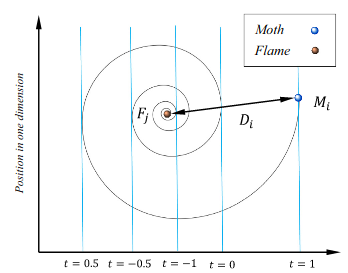
\includegraphics[width=0.4\textwidth,height=\textheight]{imgs/spiral.png}
\caption{Espiral logarítmica por la que la polilla se acerca a su
correspondiente llama}
\end{figure}

Tenemos ya definidos todos los elementos necesarios para el desarrollo
completo del algoritmo. El pseudocódigo del mismo es el que sigue:

\begin{algorithm}[H]
\DontPrintSemicolon
\SetAlgoLined
\BlankLine
    Inicializar aleatoriamente la población\;
    Evaluar la población con la función objetivo\;
    \While{No se cumpla el criterio de parada (nº iteraciones)}{
        \If{primera iteración}{
            Ordenar la población inicial por calidad\;
        } \Else {
            Juntar la población de la iteración anterior con las nuevas
            polillas\;
            Ordenar la población combinada\;
            Seleccionar una población del mismo tamaño que la original,
            formada por los mejores individuos\;
        }
        Actualizar el número de polillas en función de la iteración, N(i)\;
        Seleccionar los N(i) mejores individuos como llamas y el resto como polillas\;
        Actualizar el valor $r$ linealmente en función de la iteración\;
        \For{Cada polilla en el enjambre}{
            Generar el valor aleatorio $t$\;
            Calcular el vector director a su llama correspondiente\;
            Calcular la nueva posición con la espiral logarítmica\;
        }
    }
    Devolver el mejor individuo del conjunto y la función de pérdida en dicho punto\;
\caption{Moth-Flame Optimization Algorithm}
\end{algorithm}

Una vez hemos descrito este algoritmo de optimización, pasamos a
describir la última de las metaheurísticas estudiadas.

\hypertarget{whale-optimization-algorithm}{%
\subsection{Whale Optimization
Algorithm}\label{whale-optimization-algorithm}}

Es la metaheurística más reciente de las tres, definida en el año 2016.
Esta metaheurística se basa en el movimiento de las colonias de ballenas
cuando intentan cazar bancos de peces. Según explica el autor en la
propuesta, las ballenas cazan en grupos, comunicándose unas con otras
para informar sobre la posición de las presas por medio de ultrasonidos.
Además, una vez está localizada la presa, las ballenas se acercan a las
mismas por medio de movimientos en espiral, desde el fondo del océano y
capturando a peces que se encuentran cercanos a la superficie. Además,
algunas ballenas pueden presentar un comportamiento errático, explorando
nuevas zonas en busca de presas. Por tanto, en este caso tendremos
también tres fases diferentes en el algoritmo:

\begin{itemize}
\tightlist
\item
  Exploración del espacio de búsqueda
\item
  Comunicación con otros individuos para perseguir a las presas
\item
  Ataque en espiral
\end{itemize}

Cada una de las etapas anteriores estará determinada por un tipo de
movimiento diferente, y cada uno de estos movimientos se llevará a cabo
en una cierta etapa del algoritmo en función de una serie de
probabilidades. En primer lugar, dado que la presa viene representada
por el óptimo global de la función, el cual es desconocido a priori, se
define como presa la mejor posición encontrada hasta el momento.
Describimos los tres movimientos por separado.

\hypertarget{persecuciuxf3n-de-las-presas}{%
\subsubsection{Persecución de las
presas}\label{persecuciuxf3n-de-las-presas}}

En la persecución de las presas, las ballenas intentarán acercarse a la
presa de dicha iteración. Como hemos dicho anteriormente, la presa está
representada por la mejor solución obtenida. Las ecuaciones que marcan
dicho movimiento son las siguientes:

\[ D = \lvert C*X_p(t) - X(t) \rvert \]
\[ X(t+1) = X_p(t) - A \times D \]

Donde \(C\) y \(A\) se definen de la siguiente manera:

\[ A = 2 a r - a \] \[ C = 2 r \]

\(r\) es un vector aleatorio con componentes en el intervalo {[}0,1{]},
y \(a\) es un factor que se decrementa linealmente entre 2 y 0. Como
podemos observar, estas ecuaciones son muy similares a las que regían el
movimiento de los lobos en la búsqueda de presas.

\hypertarget{ataque-en-espiral}{%
\subsubsection{Ataque en espiral}\label{ataque-en-espiral}}

Otro de los posibles movimientos que llevan a cabo las ballenas es un
ataque en espiral rodeando a la presa. De nuevo, con \(D\) calculado de
la misma forma que en el apartado anterior, en la dirección de la presa,
la actualización del movimiento es la que sigue:

\[ X (t+1) = D* e^{bl}*cos(2 \pi l) + X_p(t) \]

Donde \(l\) es un número aleatorio en el intervalo \([-1,1]\). Como
podemos observar, este movimiento es similar al que tenían las polillas
al acercarse a las llamas.

Según el autor, las ballenas utilizan esta forma de caza
alternativamente, por lo que para decidir el movimiento de cada ballena
en una determinada iteración, se genera un número aleatorio uniforme en
el intervalo \([0,1]\), y en función de si es mayor o menor que 0.5, se
decide utilizar una ecuación de actualización de la posición u otra.

\hypertarget{buxfasqueda-de-presas}{%
\subsubsection{Búsqueda de presas}\label{buxfasqueda-de-presas}}

En último lugar, nos queda definir cómo exploran las ballenas el espacio
de búsqueda para encontrar zonas con soluciones prometedoras. En este
caso, en lugar de moverse en la dirección a la presa, la ballena se
dirige en la dirección de otra ballena aleatoria de la población,
utilizando las mismas ecuaciones que se utilizaban en la persecución a
la presa. La decisión entre un tipo de movimiento u otro (hacia la presa
o hacia otra ballena aleatoria) viene determinada por la norma del
vector \(A\). Si recuperamos su definición, \(A = 2*a*r - a\), con \(r\)
un vector aleatorio con componentes en \([0,1]\), y \(a\) un factor que
decrece linealmente entre 2 y 0. De esta manera, en las primeras etapas
del algoritmo, se espera que el vector \(A\) tenga una norma
relativamente grande, mientras que al final de la ejecución esta norma
irá tendiendo a 0. De esta manera, se decide si explorar el espacio de
búsqueda o dirigirse a cazar a una presa en función de si la norma de
\(A\) es mayor o menor que 1. Así, al principio del algoritmo, cuando la
norma del vector se espera mayor, la probabilidad de elegir la
exploración del espacio de búsqueda es alta, y posteriormente esta
probabilidad va decreciendo, mientras aumenta la probabilidad de
dirigirse a cazar a la presa.

Una vez tenemos todas las ecuaciones de movimiento definidas, podemos
listar el pseudocódigo del algoritmo:

\begin{algorithm}[H]
\DontPrintSemicolon
\SetAlgoLined
\BlankLine
    Inicializar aleatoriamente la población\;
    Evaluar la población con la función objetivo\;
    \While{No se cumpla el criterio de parada (nº iteraciones)}{
        Calcular la mejor solución, que representará a la presa\;
        Actualizar $a$\;
        \For{Cada ballena en la colonia}{
            Generar el vector aleatorio $r$, y el valor aleatorio $p$\;
            Calcular los vectores $A$ y $C$\;
            \If{|A| > 1}{
                Actualizar la posición en dirección a una ballena aleatoria\;
            } \Else {
                \If{p < 0.5} {
                    Actualizar la posición en dirección lineal a la presa\;
                } \Else {
                    Actualizar la posición hacia la presa siguiendo un ataque
                    en espiral\;
                }
            }
        }
        Comprobar si alguna ballena se ha salido de los límites del
        espacio de búsqueda y subsanarlo\;
    }
    Devolver a la presa y la función de pérdida en dicho punto\;
\caption{Whale Optimization Algorithm}
\end{algorithm}

Como podemos observar, este algoritmo guarda muchas similitudes con los
dos algoritmos anteriores. Realmente, estamos hablando de una
sofisticación de los dos algoritmos anteriores, combinándolos de forma
más o menos inteligente para tratar de eliminar posibles problemáticas
que estos presentan. Además, implementa una política nueva, que no
estaba presente en los dos primeros algoritmos de una forma tan clara, y
es la exploración aleatoria del espacio de búsqueda. En lugar de
dirigirse simplemente en la dirección de las mejores soluciones, se
permite que en las primeras etapas del algoritmo las soluciones empeoren
al dirigirse hacia soluciones aleatorias. De esta forma, se afronta en
cierta medida la posibilidad de que existan zonas prometedoras que no se
han detectado en la inicialización aleatoria.

En la siguiente sección, se describe el proceso de implementación de las
metaheurísticas que se ha llevado a cabo, así como la configuración de
la experimentación teórica.

\hypertarget{aspectos-de-implementaciuxf3n-y-ejecuciuxf3n-de-experimentos}{%
\section{Aspectos de implementación y ejecución de
experimentos}\label{aspectos-de-implementaciuxf3n-y-ejecuciuxf3n-de-experimentos}}

En esta sección se describen los aspectos de implementación del trabajo,
así como la configuración de los experimentos que se llevan a cabo. Todo
el código ha sido desarrollado en Python 3.6, utilizando como base para
cómputo la librería \texttt{numpy}. Esta librería ofrece un conjunto de
directivas para trabajar con vectores y matrices de forma eficiente,
acelerando significativamente los cálculos, ya que Python se caracteriza
por la facilidad a la hora de desarrollar código, pero a costa de ser
poco eficiente en comparación con otros lenguajes de más bajo nivel,
como C o C++.

Como se ha descrito previamente, para evaluar las metaheurísticas se va
a utilizar el conjunto de funciones de la competición CEC 2014. Para
ello, se ha encontrado una implementación de las mismas en
(\url{https://github.com/thieunguyen5991/metaheuristics/blob/master/utils/FunctionUtil.py}).
Debido a que la implementación que se ofrece aquí es relativamente poco
eficiente, se ha utilizado el esqueleto de las mismas, pero se han
modificado ciertas partes del código para optimizar los cálculos.

Para la implementación de las metaheurísticas, se ha implementado una
clase básica que actúa como interfaz, llamada \texttt{Algorithm}. Dicha
clase contiene la funcionalidad básica común para todas las
metaheurísticas, como generar una población de individuos aleatoria,
evaluar las soluciones sobre una función de pérdida, corregir soluciones
que se hayan salido de los márgenes del espacio de búsqueda, etc. Las
metaheurísticas implementadas sólo tienen que heredar de dicha clase e
implementar el método \texttt{train}. De esta manera, tenemos una
interfaz común que nos permite poder aplicar cualquier proceso de
optimización de manera sencilla. Aunque en este trabajo sólo se han
implementado metaheurísticas basadas en optimización por enjambre, la
interfaz desarrollada es genérica para cualquier tipo de metaheurística,
por lo que el código desarrollado es fácilmente extensible para permitir
la comparación de estos métodos con otros tipos de aproximaciones, como
pueden ser algoritmos genéticos, evolución diferencial, etc.

En cuanto a la configuración de la experimentación, para tratar de
realizar una comparación lo más justa posible, se ha trabajado siempre
con poblaciones de tamaño 100 para todos los algoritmos. Dado que en la
competición se fijaba de antemano el número máximo de evaluaciones de la
función objetivo, pero nuestros algoritmos funcionan a base de
iteraciones sobre la población, hemos calculado el número de iteraciones
del algoritmo como el número máximo de evaluaciones dividido entre el
tamaño de la población.

Para cada algoritmo, se han realizado 25 ejecuciones por cada función
del \emph{benchmark} para cada dimensión del problema (10, 30 y 50).
Aunque en la propuesta original se exigían 51 ejecuciones, y se
contemplaba también el problema de tamaño 100, hemos considerado
excesiva dicha experimentación, y hemos preferido reducir ligeramente
las condiciones del problema, para acelerar los cálculos. No obstante,
consideramos que 25 ejecuciones son suficientes para evaluar la robustez
de los algoritmos.

Para cada algoritmo y cada función, se mostrarán el mínimo alcanzado en
las 25 ejecuciones, el máximo, la media y la desviación típica. Se
considera que estos estadísticos son suficientes para extraer
conclusiones sobre la calidad de los algoritmos con los que se ha
trabajado.

Adicionalmente, se estudiará la velocidad de convergencia de los
algoritmos tomando la función C30, que es supuestamente la más compleja
de optimizar, para el tamaño del problema 50. Se realizarán 5
ejecuciones para cada una, y se tomarán 500 muestras del mejor valor de
la función objetivo en distintas etapas del algoritmo. Dicha información
se mostrará gráficamente para realizar un estudio comparativo.

Pasamos a mostrar el estudio de resultados obtenidos.

\hypertarget{resultados-experimentales-obtenidos}{%
\section{Resultados experimentales
obtenidos}\label{resultados-experimentales-obtenidos}}

En este apartado, mostraremos los resultados obtenidos por los tres
algoritmos sobre las treinta funciones que componen la base de datos.
Para facilitar el análisis de resultados, ya que nos encontramos ante
tablas de un tamaño considerable, vamos a dividir las funciones en
cuatro grupos, acorde con lo que se indica en la definición original del
problema:

\begin{itemize}
\tightlist
\item
  Funciones simples unimodales: Funciones 1 a 3, son funciones con un
  único punto mínimo local, que coincide con el mínimo global.
\item
  Funciones simples multimodales: Funciones 4 a 16, son funciones con
  múltiples mínimos locales, con un único punto mínimo global.
\item
  Funciones híbridas: Funciones 17 a 22, son funciones construidas a
  partir de la división del vector solución en varios fragmentos, los
  cuales se evalúan sobre algunas de las funciones simples anteriores, y
  se suman sus resultados.
\item
  Funciones compuestas: Funciones 23 a 30, similares a las anteriores,
  pero se añaden sesgos a las funciones simples para dificultar la
  obtención del mínimo.
\end{itemize}

Por la construcción de las funciones, el mínimo de cada una está en el
valor \(100i\), donde \(i\) es el índice de dicha función. Así, el
mínimo de la primera función es \(f_1(x^*) = 100\), el de la segunda
\(f_2(x^*) = 200\), y así sucesivamente. Comenzamos con los resultados
obtenidos sobre el problema de tamaño 10

\hypertarget{resultados-sobre-el-problema-de-tamauxf1o-10}{%
\subsection{Resultados sobre el problema de tamaño
10}\label{resultados-sobre-el-problema-de-tamauxf1o-10}}

A continuación se muestran las tablas de resultados para el problema de
tamaño 10:

\begin{longtable}{llrrrrr}
\caption{Resultados obtenidos en las tres primeras funciones. D = 10}\\
\toprule
   &     &     min &      50\% &       mean &         max &         std \\
\midrule
C1 & GWO & 184.195 &  539.631 &    642.621 &    1270.813 &     292.915 \\
   & MFO & 100.001 &  100.442 &    197.122 &    1027.846 &     228.963 \\
   & WOA & 121.017 &  277.264 &    286.514 &     486.201 &      95.799 \\
\midrule
C2 & GWO & 201.001 &  201.256 &    201.277 &     201.729 &       0.150 \\
   & MFO & 200.812 & 2623.667 & 476917.436 & 4673875.008 & 1290197.322 \\
   & WOA & 211.733 &  226.585 &    254.867 &     723.322 &     105.911 \\
\midrule
C3 & GWO & 305.984 &  307.802 &    307.671 &     309.249 &       0.790 \\
   & MFO & 300.000 &  300.019 &    300.995 &     312.836 &       3.078 \\
   & WOA & 304.191 &  333.367 &    335.460 &     399.305 &      26.431 \\
\bottomrule
\end{longtable}

Como podemos observar, para el grupo de funciones simples, el algoritmo
que parece arrojar un mejor comportamiento es el MFO, que consigue
quedarse a menos de una unidad del óptimo en los tres casos, si
consideramos el mínimo obtenido por los optimizadores. No obstante, si
nos fijamos en la media y la mediana de los resultados, podemos observar
que este algoritmo se comporta de forma poco robusta para la función C2,
donde rápidamente empieza a sufrir un empeoramiento notable. El
optimizador basado en manadas de lobos parece ser el más estable en las
funciones 2 y 3, como se refleja en la desviación típica de los
resultados. Por otra parte, WOA es el algoritmo más estable en general,
aunque los resultados que obtiene no son especialmente buenos en ningún
caso. Los resultados parecen mostrar que WOA es el algoritmo que se
comporta bien en un contexto amplio de funciones, mientras que los otros
dos optimizadores consiguen grandes resultados en algunos casos, pero
tienden a ser menos robustos.

Pasamos a ver el siguiente grupo de funciones:

\begin{longtable}{llrrrrr}
\caption{Resultados obtenidos sobre el segundo grupo de funciones. D = 10} \\
\toprule
    &     &      min &      50\% &     mean &      max &     std \\
\midrule
C4 & GWO &  400.001 &  401.217 &  400.929 &  401.431 &   0.494 \\
    & MFO &  403.143 &  407.327 &  407.184 &  409.606 &   1.744 \\
    & WOA &  400.000 &  400.000 &  400.000 &  400.002 &   0.001 \\
\midrule
C5 & GWO &  500.001 &  502.056 &  501.662 &  502.872 &   0.887 \\
    & MFO &  520.000 &  520.014 &  520.020 &  520.121 &   0.027 \\
    & WOA &  500.000 &  500.011 &  500.404 &  503.223 &   0.845 \\
\midrule
C6 & GWO &  600.000 &  600.000 &  600.000 &  600.000 &   0.000 \\
    & MFO &  600.000 &  603.667 &  602.804 &  605.717 &   2.208 \\
    & WOA &  600.000 &  600.000 &  600.000 &  600.000 &   0.000 \\
\midrule
C7 & GWO &  700.085 &  700.178 &  700.177 &  700.284 &   0.052 \\
    & MFO &  700.017 &  700.108 &  700.149 &  700.571 &   0.133 \\
    & WOA &  700.046 &  700.149 &  700.191 &  700.522 &   0.125 \\
\midrule
C8 & GWO &  800.000 &  800.000 &  800.021 &  800.516 &   0.103 \\
    & MFO &  802.985 &  809.950 &  809.997 &  818.907 &   4.572 \\
    & WOA &  800.000 &  800.000 &  800.160 &  801.003 &   0.374 \\
\midrule
C9 & GWO &  900.000 &  900.000 &  900.041 &  900.516 &   0.143 \\
    & MFO &  903.981 &  911.958 &  913.361 &  934.868 &   7.938 \\
    & WOA &  900.000 &  900.000 &  900.080 &  901.004 &   0.277 \\
\midrule
C10 & GWO & 1000.000 & 1000.000 & 1000.500 & 1012.506 &   2.501 \\
    & MFO & 1075.048 & 1962.041 & 1951.266 & 2709.050 & 416.630 \\
    & WOA & 1000.000 & 1000.663 & 1009.673 & 1122.234 &  24.678 \\
\midrule
C11 & GWO & 1100.000 & 1100.000 & 1100.500 & 1112.506 &   2.501 \\
    & MFO & 1200.029 & 2035.908 & 2027.484 & 2674.896 & 374.419 \\
    & WOA & 1100.001 & 1100.096 & 1103.083 & 1130.431 &   7.087 \\
\midrule
C12 & GWO & 1200.001 & 1200.022 & 1200.026 & 1200.078 &   0.021 \\
    & MFO & 1200.000 & 1200.000 & 1200.000 & 1200.000 &   0.000 \\
    & WOA & 1200.004 & 1200.472 & 1200.705 & 1202.029 &   0.573 \\
\midrule
C13 & GWO & 1300.253 & 1300.369 & 1300.369 & 1300.514 &   0.063 \\
    & MFO & 1300.048 & 1300.215 & 1300.203 & 1300.435 &   0.102 \\
    & WOA & 1300.185 & 1300.397 & 1300.377 & 1300.579 &   0.105 \\
\midrule
C14 & GWO & 1400.280 & 1400.454 & 1400.436 & 1400.497 &   0.063 \\
    & MFO & 1400.176 & 1400.245 & 1400.258 & 1400.415 &   0.058 \\
    & WOA & 1400.057 & 1400.159 & 1400.156 & 1400.252 &   0.052 \\
\midrule
C15 & GWO & 1500.000 & 1500.023 & 1500.055 & 1500.296 &   0.081 \\
    & MFO & 1500.127 & 1500.542 & 1500.631 & 1501.635 &   0.402 \\
    & WOA & 1500.000 & 1500.114 & 1500.195 & 1501.303 &   0.287 \\
\midrule
C16 & GWO & 1600.000 & 1600.823 & 1600.747 & 1600.824 &   0.188 \\
    & MFO & 1600.819 & 1600.983 & 1601.276 & 1602.329 &   0.514 \\
    & WOA & 1600.000 & 1600.685 & 1600.669 & 1602.181 &   0.629 \\
\bottomrule
\end{longtable}

Para este grupo de funciones, los resultados parecen ser bastante
adecuados. Los tres algoritmos son capaces de acercarse
significativamente al mínimo en prácticamente todas las funciones. El
únicos valores que pueden resultar anormalmente altos son los que
obtiene MFO sobre la función 11, que se queda a 100 unidades del mínimo,
y en la función 10, que se queda a 75 puntos. El resto de ejecuciones
obtienen resultados muy adecuados en cuanto al valor mínimo. En muchos
casos, incluso el valor máximo (correspondiente a la peor ejecución),
sólo se queda a escasas unidades del óptimo, lo que indica que los
algoritmos se comportan especialmente bien en este grupo de funciones.
En particular, WOA y GWO consiguen alcanzar el valor óptimo de la
función C6 en sus 25 ejecuciones, y MFO lo hace para la función C12.

Analizando globalmente los algoritmos, parece que MFO es el que peor se
comporta en este grupo de funciones, y es el menos robusto de los tres
algoritmo. La desviación típica de sus ejecuciones suele ser
significativamente más alta que la de las otras dos metaheurísticas, y
los valores de la función que alcanza son ligeramente más altos. GWO y
WOA parecen tener un comportamiento más o menos similar, y resulta
difícil establecer cuál de los dos algoritmos tiene mejor
comportamiento. Sus resultados son muy similares en todos los
estadísticos extraídos, siendo quizás ligeramente peores los de WOA en
algunos aspectos, pero de forma poco significativa (puede observarse por
ejemplo que en C10 el comportamiento de WOA es ligeramente peor que el
de GWO, dado que la media, el máximo y la desviación típica son más
altas en WOA).

Pasamos a observar el primer grupo de funciones compuestas:

\begin{longtable}{llrrrrr}
\caption{Resultados obtenidos sobre el tercer grupo de funciones. D = 10} \\
\toprule
    &     &      min &      50\% &     mean &       max &      std \\
\midrule
C17 & GWO & 1703.889 & 1704.380 & 1708.239 &  1736.001 &    9.290 \\
    & MFO & 1700.000 & 1704.984 & 1730.605 &  1922.262 &   64.640 \\
    & WOA & 1701.037 & 1717.645 & 1718.903 &  1750.629 &   13.569 \\
\midrule
C18 & GWO & 1805.073 & 1805.593 & 1806.869 &  1818.131 &    3.013 \\
    & MFO & 1800.492 & 1810.428 & 1812.372 &  1842.913 &    9.670 \\
    & WOA & 1823.451 & 2027.193 & 2133.306 &  2782.722 &  286.910 \\
\midrule
C19 & GWO & 1901.247 & 1901.728 & 1901.922 &  1905.458 &    0.838 \\
    & MFO & 1901.551 & 1902.940 & 1908.959 &  1957.303 &   14.068 \\
    & WOA & 1901.011 & 1905.421 & 1921.064 &  1999.764 &   29.603 \\
\midrule
C20 & GWO & 2004.070 & 2020.588 & 2021.448 &  2046.107 &   14.014 \\
    & MFO & 2001.021 & 2002.469 & 2004.932 &  2024.023 &    5.042 \\
    & WOA & 2017.279 & 2074.714 & 3243.148 & 14379.682 & 2971.426 \\
\midrule
C21 & GWO & 2102.261 & 2105.258 & 2104.631 &  2106.916 &    1.504 \\
    & MFO & 2100.084 & 2103.207 & 2128.306 &  2335.819 &   61.495 \\
    & WOA & 2101.863 & 2120.803 & 2380.289 &  5334.219 &  818.717 \\
\midrule
C22 & GWO & 2200.123 & 2200.272 & 2204.919 &  2220.012 &    8.523 \\
    & MFO & 2200.033 & 2220.197 & 2217.602 &  2220.977 &    6.584 \\
    & WOA & 2200.077 & 2200.617 & 2204.927 &  2220.778 &    7.964 \\
\bottomrule
\end{longtable}

Para este conjunto de funciones podemos observar un comportamiento
similar al que tuvimos al principio, en el que MFO resultaba ser el
mejor de los algoritmos a la hora de alcanzar el mínimo, pero luego
resultaba ser poco estable. Podemos observar que, a pesar de ser el
algoritmo que mejores resultados obtiene cuando observamos el mínimo, se
ve ampliamente superado por GWO para casi todas las funciones cuando
comprobamos el máximo, lo cual significa que GWO es más estable. Resulta
curioso observar el mal comportamiento que presenta aquí WOA, que
consigue unos resultados bastante pobres en términos de estabilidad,
como puede observarse a partir de la desviación típica de sus
resultados.

Pasamos al último grupo de funciones.

\begin{longtable}{llrrrrr}
\caption{Resultados obtenidos sobre el último grupo de funciones. D = 10} \\
\toprule
    &     &      min &       50\% &      mean &       max &       std \\
\midrule
C23 & GWO & 2300.565 &  2300.608 &  2300.604 &  2300.632 &     0.018 \\
    & MFO & 2300.733 &  2310.389 &  2323.506 &  2380.343 &    25.897 \\
    & WOA & 2300.967 &  2301.290 &  2301.374 &  2302.180 &     0.323 \\
\midrule
C24 & GWO & 2400.022 &  2400.036 &  2403.949 &  2448.948 &    13.543 \\
    & MFO & 2614.142 &  2728.300 &  2793.511 &  3072.754 &   136.827 \\
    & WOA & 2400.328 &  2400.705 &  2404.956 &  2489.958 &    17.949 \\
\midrule
C25 & GWO & 2500.022 &  2500.041 &  2501.732 &  2542.280 &     8.448 \\
    & MFO & 2670.091 &  2698.879 &  2692.284 &  2700.067 &    11.018 \\
    & WOA & 2500.243 &  2500.560 &  2500.652 &  2501.909 &     0.329 \\
\midrule
C26 & GWO & 2600.037 &  2600.068 &  2600.071 &  2600.100 &     0.018 \\
    & MFO & 2798.260 &  2826.263 &  2827.448 &  2879.085 &    19.835 \\
    & WOA & 2600.517 &  2600.835 &  2600.881 &  2601.886 &     0.276 \\
\midrule
C27 & GWO & 2705.048 &  2705.070 &  2708.077 &  2780.219 &    15.030 \\
    & MFO & 3044.032 &  3051.756 &  3052.736 &  3070.403 &     5.137 \\
    & WOA & 2705.546 &  2706.165 &  2706.159 &  2706.849 &     0.371 \\
\midrule
C28 & GWO & 3256.246 &  3513.456 &  3489.406 &  3565.133 &    71.231 \\
    & MFO & 3189.123 &  3191.600 &  3191.742 &  3194.162 &     1.233 \\
    & WOA & 2801.130 &  2801.609 &  2809.363 &  2911.129 &    26.190 \\
\midrule
C29 & GWO & 3331.107 &  3621.242 &  4806.800 &  7376.930 &  1647.233 \\
    & MFO & 3101.795 &  3118.867 &  3145.981 &  3649.500 &   108.917 \\
    & WOA & 3043.539 & 10912.608 &  9856.720 & 16463.023 &  3776.045 \\
\midrule
C30 & GWO & 3102.647 &  3196.122 &  3192.124 &  3259.085 &    42.237 \\
    & MFO & 3220.064 &  3220.636 &  3223.838 &  3237.215 &     6.779 \\
    & WOA & 3040.212 &  3218.649 & 10388.001 & 68136.200 & 17201.162 \\
\bottomrule
\end{longtable}

Comentamos los resultados sobre el último grupo de funciones. Por un
lado, aquí podemos observar que el optimizador que mejores resultados
obtiene es WOA en términos del mínimo, por lo que parece que para
funciones más complejas es el optimizador más adecuado. Podemos observar
que ahora MFO sí que tiene una pérdida de rendimiento importante, y se
queda lejos del mínimo para muchas de las funciones. De la misma manera,
GWO queda lejos del óptimo en las últimas 3 funciones. WOA, por el
contrario, se queda bastante cerca en todos los casos, a excepción de la
función C29, que la mejor ejecución global está a más de 100 puntos del
mínimo. En cuanto a la estabilidad de las soluciones, WOA y GWO
presentan un comportamiento bastante adecuado en general, a excepción de
las dos últimas funciones, en las que la desviación típica se dispara.
MFO, aunque con peor rendimiento en general, no sufre de esos repuntes
tan bruscos en ninguna ejecución. Resulta especialmente preocupante el
peor resultado obtenido por WOA en las dos últimas funciones, que llega
a obtener valores del orden de 60000, lo cual está muy alejado del
mínimo a alcanzar. Aquí puede vislumbrarse uno de los principales
problemas que tienen los modelos de optimización basados en poblaciones.
Aunque la probabilidad de obtener unos resultados tan malos es bastante
baja, existe la posibilidad de que el resultado quede muy lejos del
óptimo de la función. Es por esto por lo que, cuando se utilizan estos
optimizadores en la resolución de problemas reales, se recomiende
ejecutar los mismos varias veces, para eliminar en parte la componente
aleatoria que los gobierna.

\hypertarget{referencias}{%
\section*{Referencias}\label{referencias}}
\addcontentsline{toc}{section}{Referencias}

\hypertarget{refs}{}
\leavevmode\hypertarget{ref-kennedy1995particle}{}%
Kennedy, James, and Russell Eberhart. 1995. ``Particle Swarm
Optimization.'' In \emph{Proceedings of Icnn'95-International Conference
on Neural Networks}, 4:1942--8. IEEE.

\leavevmode\hypertarget{ref-liang2013problem}{}%
Liang, JJ, BY Qu, and PN Suganthan. 2013. ``Problem Definitions and
Evaluation Criteria for the Cec 2014 Special Session and Competition on
Single Objective Real-Parameter Numerical Optimization.''
\emph{Computational Intelligence Laboratory, Zhengzhou University,
Zhengzhou China and Technical Report, Nanyang Technological University,
Singapore} 635.

\leavevmode\hypertarget{ref-mirjalili2015moth}{}%
Mirjalili, Seyedali. 2015. ``Moth-Flame Optimization Algorithm: A Novel
Nature-Inspired Heuristic Paradigm.'' \emph{Knowledge-Based Systems} 89:
228--49.

\leavevmode\hypertarget{ref-mirjalili2016whale}{}%
Mirjalili, Seyedali, and Andrew Lewis. 2016. ``The Whale Optimization
Algorithm.'' \emph{Advances in Engineering Software} 95: 51--67.

\leavevmode\hypertarget{ref-mirjalili2014grey}{}%
Mirjalili, Seyedali, Seyed Mohammad Mirjalili, and Andrew Lewis. 2014.
``Grey Wolf Optimizer.'' \emph{Advances in Engineering Software} 69:
46--61.

\end{document}
